%本章证明优化潜力的存在性

\chapter{优化潜力存在性}
\label{chapter:优化潜力}

在本章中,我们将忽略相关性和提前期等一切影响因素,单纯从需求的概率分布变化来探究在制品库存前置策略对安全库存的优化作用。






\section{安全库存的制定标准}

(此处待补充一些文献,详细讨论什么是安全库存)

安全库存的计算方式是总库存减去需求的期望值。由于本文讨论的所有情况都不涉及需求期望值的变动,因此在比较策略实施前后安全库存的变化时,总库存的减少量与安全库存的减少量始终是等价的。本文后续讨论中不再刻意强调安全库存与总库存的区别,以减少繁琐的数学表达,使数学公式的推导更简洁。

在讨论安全库存时,我们常用的标准有惩罚成本和服务水平。

惩罚成本是企业在缺货时需要付出的成本。合同罚款就是最常见的惩罚成本之一。在汽车配件的生产过程中,配件生产商会和需求方签订合同,当生产商不能按时供货时,就需要承受一笔罚款。惩罚成本能够比较直观地反应缺货带来的损失,体现安全库存的作用。

然而,惩罚成本在使用过程中有一个难以解决的问题:如何准确确定惩罚成本。惩罚成本不仅包括实际的资金损失,还应该考虑其他隐性损失。以汽车配件生产商为例,合同规定的罚款只是表面上的惩罚成本,实际的损失还应该包括企业的声誉损失。汽车行业非常重视精益生产,缺货造成的声誉损失可能使企业丢失更多的潜在订单,甚至失去合作伙伴。这些损失比表面上的罚款更严重,但很难对其进行量化。

因此,如果仅仅使用合同的罚款数额作为惩罚成本,那么分析过程使用的惩罚成本是小于实际损失的。这种情况下,企业做出的决策,会更倾向于承受损失。这是对企业有害的。

本文中,我们将主要使用服务水平作为安全库存的制定标准。这样做的原因不仅包括以上讨论的惩罚成本的缺陷,还有给出更为科学的理由。在接下来的论述中,我们将会证明,如果使用惩罚成本作为安全库存的制定标准,与使用服务水平相比,并不能带来更多的优势。

若只考虑惩罚成本,不考虑库存成本,则企业需要设定一个自己能接受的惩罚成本期望的最大值。我们首先分析惩罚成本的期望。设企业的库存为$K$,惩罚成本为$p$,需求服从分布$P(X=x)=f(x)$,其累积分布为$P(X<x)=F(x)$。则惩罚成本为
\begin{equation}
C(x,K)=\left\{
\begin{aligned}
&0, &x \leq K \\
&p(x-K), &x > K
\end{aligned}
\right.
\label{eq:惩罚成本}
\end{equation}
如果期望存在的话,其对应的期望是
\begin{align}
E[C(x,K)] &= \int_{-\infty}^{+\infty}C(x,K)f(x)\dif x\notag\\
&=\int_K^{+\infty}p(x-K)f(x)\dif x\notag\\
&=p(x-K)F(x)\bigg|_K^{+\infty} - \int_K^{+\infty}pF(x)\dif x\notag\\
&=\lim_{M\to+\infty}\left[p(M-K) - \int_K^MpF(x)\dif x\right]\notag\\
&=\lim_{M\to+\infty}\left[\int_K^Mp\dif x - \int_K^MpF(x)\dif x\right]\notag\\
&=p\int_K^{+\infty}(1-F(x))\dif x
\label{eq:惩罚成本期望}
\end{align}
另一方面,库存为$K$时,对应的服务水平是
\begin{equation}
\eta = \int_{-\infty}^Kf(x)\dif x
\label{eq:服务水平}
\end{equation}

由公式\ref{eq:惩罚成本期望}和\ref{eq:服务水平}可知,惩罚成本期望是随$K$单调递减的,服务水平是随$K$单调递增的。二者可以一一对应,即每个惩罚成本期望值都对应某个特定的服务水平。企业制定自己的惩罚成本期望值,和制定自己的服务水平,是等价的。

使用服务水平来计算安全库存时,不需要考虑库存成本。使用惩罚成本时,可以把库存成本也加入到模型中。接下来我们将证明,加入库存成本之后,惩罚成本与服务水平是一一对应的。以下推导过程中使用离散的库存量和需求量。

设企业的库存为$K$,需求为$D$,惩罚成本为$p$,库存成本为$h$。则总成本为
\begin{equation}
C(K) = p\max\{D-K,0\} + h(\frac{1}{2}\min\{D,K\}+\max\{K-D,0\})
\label{eq:库存和惩罚成本}
\end{equation}
企业的目标是寻找最优的库存$K$,使得库存成本和惩罚成本之和的期望最小。我们对公式\ref{eq:库存和惩罚成本}中的几个部分分别求期望。
\begin{align}
E(\min\{D,K\}) &= \sum_{i=1}^{\infty}\min\{i,K\}P(D=i) \notag\\
&= \sum_{i=1}^{\infty}\sum_{j=1}^{\min\{i,K\}}P(D=i) \notag\\
&= \sum_{j=1}^K\sum_{i=j}^{\infty}P(D=i) \notag\\
&= \sum_{j=1}^K P(D \geq j) \label{eq:期望1}\\
E(\max\{D-K,0\}) &= -\min\{K-D,0\} \notag\\
&= -(\min\{K,D\}-D) \notag\\
&= D - \sum_{j=1}^K P(D \geq j) \label{eq:期望2}\\
E(\max\{K-D,0\}) &= \sum_{i=1}^{\infty}\max\{K-i,0\}P(D=i) \notag\\
&= \sum_{i=1}^{\infty}\sum_{j=1}^{\max\{K-i,0\}}P(D=i) \notag\\
&= \sum_{j=1}^{K-1}\sum_{i=1}^j P(D=i) \notag\\
&= \sum_{j=1}^{K-1}P(D \leq j) \label{eq:期望3}
\end{align}
将公式\ref{eq:期望1}、\ref{eq:期望2}和\ref{eq:期望3}代入公式\ref{eq:库存和惩罚成本}可得
\begin{equation}
E[C(K)] = pD + (\frac{h}{2}-p)\sum_{j=1}^K P(D \geq j) + h\sum_{j=1}^{K-1} P(D \leq j)
\label{eq:库存和惩罚成本期望}
\end{equation}
考虑库存增加时,总成本的增量
\begin{align}
E[C(K+1)]-E[C(K)] &= (\frac{h}{2}-p)P(D\geq K+1) + hP(D\leq K) \notag\\
&= \frac{h}{2}-p+(\frac{h}{2}+p)P(D\leq K) \label{eq:总成本增量}
\end{align}
公式\ref{eq:总成本增量}是随$K$单调递增的,因此,当$E[C(K+1)]-E[C(K)]$取得0值时,$E[C(K)]$取得最小值。此时有
\begin{equation}
P(D\leq K) = \frac{2p-h}{2p+h}
\label{eq:惩罚成本与服务水平的关系}
\end{equation}
其中$P(D\leq K)$即等于企业的服务水平$\eta$。本文讨论的库存策略仅移动在制品库存在生产线上的位置,不影响库存费用和需求分布。因此,给出任意的惩罚成本,都有一个唯一的服务水平与之对应。

通过以上的讨论,我们已经证明了,以惩罚成本和库存成本来制定安全库存的问题,可以转化为以服务水平来制定安全库存的问题。为了使数学推导更加简洁,本文余下的部分将主要使用服务水平作为安全库存的制定标准。企业可以根据实际情况选取合适的制定方式,且不影响本文中结论的适用性。












\section{两种成品需求独立正态分布}

仍然以汽车保险杠生产为例,假设某种汽车保险杠只有两种颜色,且两种颜色的需求服从独立的正态分布。第一种颜色的保险杠,需求$D_1$服从正态分布$N_1(\mu_1,\sigma_1^2)$;第二种颜色的保险杠,需求$D_2$服从正态分布$N_2(\mu_2,\sigma_2^2)$。企业设定的服务水平为$\eta$。设$z_\eta$是标准正态分布的$\eta$分位数,即$z_\eta$满足
\[
\int_{-\infty}^{z_\eta}\frac{1}{\sqrt{2\pi}}e^{-\frac{x^2}{2}}\dif x = \eta
\]
则此服务水平下,两种成品的库存分别为
\begin{align}
\xi_1 &= \mu_1 + z_\eta\sigma_1 \label{eq:成品库存1}\\
\xi_2 &= \mu_2 + z_\eta\sigma_2 \label{eq:成品库存2}
\end{align}

现在假设我们按照改进策略,取消两种颜色的成品库存,改为保留未喷涂的在制品库存。忽略供货提前期等变化的影响。企业的服务水平仍然为$\eta$。为了满足该服务水平,所需的在制品库存为$\xi$。此时的在制品库存需要同时应对两种颜色的成品需求,因此,对未喷涂的在制品需求为$D=D_1+D_2$。

设$D_1$、$D_2$的联合分布为$f(x_1,x_2)$。因为$D_1$、$D_2$是独立的,所以$f(x_1,x_2)$的概率分布为
\begin{align}
f(x_1,x_2) &= f(x_1)\cdot f(x_2) \notag\\
&= \frac{1}{\sqrt{2\pi}\sigma_1}e^{-\frac{(x_1-\mu_1)^2}{2\sigma_1^2}}\cdot \frac{1}{\sqrt{2\pi}\sigma_2}e^{-\frac{(x_2-\mu_2)^2}{2\sigma_2^2}} \notag\\
&= \frac{1}{2\pi\sigma_1\sigma_2}e^{-\frac{1}{2}\left[\frac{(x_1-\mu_1)^2}{\sigma_1^2}+\frac{(x_2-\mu_2)^2}{\sigma_2^2}\right]}
\label{eq:联合分布}
\end{align}

设$D$、$D_2$的联合分布为$g(y_1,y_2)$。由$y_1=x_1+x_2,y_2=x_2$得$x_1=y_1-y_2,x_2=y_2$。因此,雅可比矩阵为
\[
J = \begin{bmatrix}
\frac{\partial x_1}{\partial y_1} & \frac{\partial x_1}{\partial y_2} \\
\frac{\partial x_2}{\partial y_1} & \frac{\partial x_2}{\partial y_2}
\end{bmatrix} = \begin{bmatrix}
1 & -1 \\
0 & 1
\end{bmatrix}
\]
由此可得$g(y_1,y_2)$的概率分布为
\begin{align}
g(y_1,y_2) &= f(x_1,x_2)\cdot\left|J\right| \notag\\
&= f(y_1-y_2,y_2)\cdot
\begin{vmatrix}
1 & -1 \\
0 & 1
\end{vmatrix} \notag\\
&= \frac{1}{2\pi\sigma_1\sigma_2}e^{-\frac{1}{2}\left[\frac{(y_1-y_2-\mu_1)^2}{\sigma_1^2}+\frac{(y_2-\mu_2)^2}{\sigma_2^2}\right]}
\label{eq:新联合分布}
\end{align}
$g(y_1,y_2)$的边缘分布$h(y_1)$即是在制品需求$D$的概率分布。对$y_2$积分可得
\begin{equation}
h(y_1) = \int_{-\infty}^{+\infty}\frac{1}{2\pi\sigma_1\sigma_2}e^{-\frac{1}{2}\left[\frac{(y_1-y_2-\mu_1)^2}{\sigma_1^2}+\frac{(y_2-\mu_2)^2}{\sigma_2^2}\right]}\dif y_2
\label{eq:求边缘分布}
\end{equation}
令
\[
A = \frac{1}{\sqrt{2\pi(\sigma_1^2+\sigma_2^2)}}e^{-\frac{[y_1-(\mu_1+\mu_2)]^2}{2(\sigma_1^2+\sigma_2^2)}}
\]
则公式\ref{eq:求边缘分布}可变形为
\begin{align}
h(y_1) &= A\int_{-\infty}^{+\infty}\frac{\sqrt{2\pi(\sigma_1^2+\sigma_2^2)}}{2\pi\sigma_1\sigma_2}e^{-\frac{1}{2}\left[\frac{(y_1-y_2-\mu_1)^2}{\sigma_1^2}+\frac{(y_2-\mu_2)^2}{\sigma_2^2}\right]+\frac{[y_1-(\mu_1+\mu_2)]^2}{2(\sigma_1^2+\sigma_2^2)}}\dif y_2 \notag\\
&= A\int_{-\infty}^{+\infty}\frac{\sqrt{\sigma_1^2+\sigma_2^2}}{\sqrt{2\pi}\sigma_1\sigma_2}e^{-\frac{1}{2}\left[\frac{\sqrt{\sigma_1^2+\sigma_2^2}}{\sigma_1\sigma_2}y_2-\left(\frac{\sigma_2}{\sigma_1\sqrt{\sigma_1^2+\sigma_2^2}}(y_1-\mu_1)+\frac{\sigma_1}{\sigma_2\sqrt{\sigma_1^2+\sigma_2^2}}\mu_2\right)\right]^2}\dif y_2
\label{eq:求边缘分布2}
\end{align}
再令
\[
t = \frac{\sqrt{\sigma_1^2+\sigma_2^2}}{\sigma_1\sigma_2}y_2-\left(\frac{\sigma_2}{\sigma_1\sqrt{\sigma_1^2+\sigma_2^2}}(y_1-\mu_1)+\frac{\sigma_1}{\sigma_2\sqrt{\sigma_1^2+\sigma_2^2}}\mu_2\right)
\]
则公式\ref{eq:求边缘分布2}可变形为
\begin{equation}
h(y_1) = A\int_{-\infty}^{+\infty}\frac{1}{\sqrt{2\pi}}e^{-\frac{t^2}{2}}\dif t
\label{eq:求边缘分布3}
\end{equation}
公式\ref{eq:求边缘分布3}的右半部分是标准正态分布的累积概率函数,总累积概率应该为1,即
\[
\int_{-\infty}^{+\infty}\frac{1}{\sqrt{2\pi}}e^{-\frac{t^2}{2}}\dif t = 1
\]
因此得到$h(y_1)=A$,即
\begin{equation}
h(y_1) = \frac{1}{\sqrt{2\pi(\sigma_1^2+\sigma_2^2)}}e^{-\frac{[y_1-(\mu_1+\mu_2)]^2}{2(\sigma_1^2+\sigma_2^2)}}
\label{eq:边缘分布结果}
\end{equation}

由公式\ref{eq:边缘分布结果}可知,在制品的需求$D$服从正态分布$N(\mu_1+\mu_2,\sigma_1^2+\sigma_2^2)$。为了满足服务水平$\eta$,所需的在制品库存为
\begin{equation}
\xi = \mu_1 + \mu_2 + z_\eta\sqrt{\sigma_1^2+\sigma_2^2}
\label{eq:在制品库存}
\end{equation}

至此,我们可以利用公式\ref{eq:成品库存1}、\ref{eq:成品库存2}和\ref{eq:在制品库存}将改进前后的库存总量进行比较
\begin{align}
\xi_1 + \xi_2 - \xi &= \mu_1 + z_\eta\sigma_1 + \mu_2 + z_\eta\sigma_2 - \left(\mu_1 + \mu_2 + z_\eta\sqrt{\sigma_1^2+\sigma_2^2}\right) \notag\\
&= z_\eta\left(\sigma_1+\sigma_2-\sqrt{\sigma_1^2+\sigma_2^2}\right) \notag\\
&> z_\eta\left(\sigma_1+\sigma_2-\sqrt{\sigma_1^2+\sigma_2^2+2\sigma_1\sigma_2}\right) \notag\\
&= z_\eta\left(\sigma_1+\sigma_2-\sqrt{(\sigma_1+\sigma_2)^2}\right) \notag\\
&= 0
\label{eq:改进前后库存比较}
\end{align}
由公式\ref{eq:改进前后库存比较}可知$\xi_1+\xi_2>\xi$,即改进后的在制品库存严格小于改进前的成品库存之和。这个结果说明,当两种不同颜色的成品需求服从独立正态分布时,通过保留在制品库存能够降低企业的库存总量。



\section{两种以上的成品需求独立正态分布}

现在我们将上述结果进行推广。假设某种汽车保险杠有$N$种颜色($N\geq 2$),并且服从两两相互独立的正态分布。第$i$种颜色的保险杠,需求$D_i$服从正态分布$N_i(\mu_i,\sigma_i^2)$,$i=1,2,\ldots,N$。企业的服务水平仍为$\eta$,其对应的标准正态分布$\eta$分位数仍为$z_\eta$。

为了满足此服务水平,各成品需要保留的库存为
\begin{equation}
\xi_i = \mu_i + z_\eta\sigma_i,\qquad i=1,2,\ldots,N
\label{eq:成品库存i}
\end{equation}

现在假设我们按照改进策略,取消所有颜色的成品库存,改为保留未喷涂的在制品库存。为了满足服务水平$\eta$,所需的在制品库存为$\xi$。此时在制品库存的需求为$D=\sum_{i=1}^ND_i$。前面已证任意两个独立的正态分布之和仍然服从正态分布,由于所有的$D_i$都是相互独立的,因此它们可以连续加和,其结果仍然服从正态分布。所以我们有$D\sim N(\sum_{i=1}^N\mu_i,\sum_{i=1}^N\sigma_i^2)$。进而可以得到在制品库存为
\begin{equation}
\xi = \sum_{i=1}^N\mu_i + z_\eta\sqrt{\sum_{i=1}^N\sigma_i^2}
\label{eq:在制品库存i}
\end{equation}

通过公式\ref{eq:成品库存i}和\ref{eq:在制品库存i}比较改进前后的库存变化
\begin{align}
\sum_{i=1}^N\xi_i - \xi &= \sum_{i=1}^N (\mu_i+z_\eta\sigma_i) - \left(\sum_{i=1}^N\mu_i + z_\eta\sqrt{\sum_{i=1}^N\sigma_i^2}\right) \notag\\
&= z_\eta\left(\sum_{i=1}^N\sigma_i-\sqrt{\sum_{i=1}^N\sigma_i^2}\right) \notag\\
&> z_\eta\left(\sum_{i=1}^N\sigma_i-\sqrt{\sum_{i=1}^N\sigma_i^2+2\sum_{i=1}^{N-1}\sum_{j=i+1}^N\sigma_i\sigma_j}\right) \notag\\
&= z_\eta\left(\sum_{i=1}^N\sigma_i-\sqrt{\left(\sum_{i=1}^N\sigma_i\right)^2}\right) \notag\\
&= 0
\label{eq:改进前后库存比较i}
\end{align}
由公式\ref{eq:改进前后库存比较i}可知$\sum_{i=1}^N\xi_i > \xi$,即改进后的在制品库存严格小于改进前的成品库存。至此,我们已证明,当成品库存服从两两相互独立的正态分布时,通过保留在制品库存能够降低企业的库存总量。








\section{一些参数对改进效果的影响}

前面已经证明了保留在制品库存的改进能够达到降低安全库存的目的,本节将讨论影响改进效果的参数,找出最适宜进行改进的环境。

到目前为止,我们探讨的过程中出现过的参数主要有需求的均值、方差和企业的服务水平。其中,需求的均值决定的是库存中固定的部分而非波动的部分,因此需求均值对于改进效果是没有影响的。我们需要考虑的是需求的方差和企业的服务水平对改进效果的影响。

为了使问题更简单,我们假设只有两种成品参与改进,它们的需求相互独立,且都服从相同的正态分布$N(\mu,\sigma^2)$。由公式\ref{eq:边缘分布结果}可知,改进后的需求服从正态分布$N(2\mu,2\sigma^2)$。企业的服务水平为$\eta$,则改进前的安全库存为$2\cdot z_{\eta}\cdot\sigma$,改进后的安全库存为$z_{\eta}\cdot\sqrt{2}\sigma$。每一个标准差$\sigma$和每一个服务水平$\eta$,都对应着一个改进前后的库存差值$\Delta=2z_{\eta}\sigma-\sqrt{2}z_{\eta}\sigma$。利用计算机程序求出$\sigma\in[0,50]$、$\eta\in(0,1)$的所有对应$\Delta$值,并作图如图\ref{fig:需求波动和服务水平对改进效果的影响}所示。

\begin{figure}[htb]
\centering
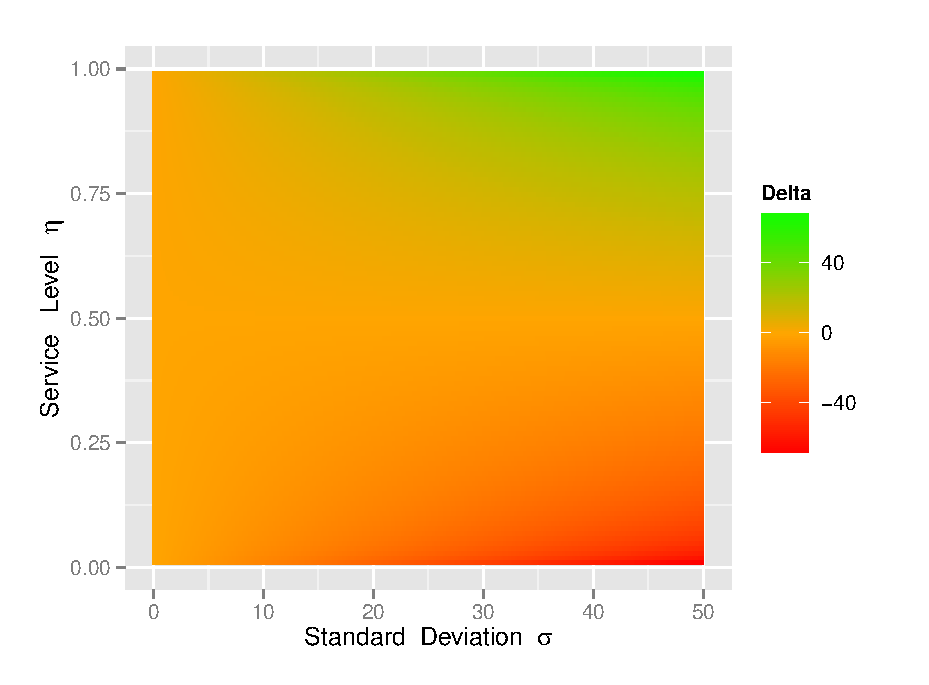
\includegraphics[width=15cm]{normal_effect.eps}
\caption{需求波动和服务水平对改进效果的影响}
\label{fig:需求波动和服务水平对改进效果的影响}
\end{figure}

图\ref{fig:需求波动和服务水平对改进效果的影响}中每个点的位置代表一种$(\sigma,\eta)$组合,每个点的颜色代表该处的$\Delta$值。颜色越绿,代表改进效果越好;颜色越红,代表改进效果越差。

观察图中颜色的分布区域和渐变趋势,可以得到以下结论:
\begin{enumerate}
\item 绿色区域集中在右上角,并向右上方渐变,说明需求波动大、企业服务水平高的环境下,改进效果是最好的,改进策略值得考虑;
\item 红色区域集中在右下角,并向右下方渐变,说明需求波动大、企业服务水平低的环境下,改进效果是最差的,改进之前需要慎重;
\item 需求波动相同的情况下,企业服务水平越高,改进的效果越好;
\item 企业服务水平相同的情况下,需求的波动越强,改进的效果越好。
\end{enumerate}

除此之外还能发现,在$\eta=0.5$处出现了一条疑似“对称轴”,并且该轴两侧的改进效果竟然有正负之别。下一章中,我们将详细讨论这个问题。










